\subsection{Continuous-time methods}
\label{m:sec:methct}

The continuous-time stock is larger, and this subsection develops it with the
linear birth--death process of \cref{m:sec:linbd} as the running example:
backward equations, mean population size, variance and higher moments, hitting
probabilities, extinction probabilities, and conditional means. Every item has
a discrete-time counterpart in \cref{m:sec:methdisc}, and the correspondences
are pointed out as they arise. The one item that has no discrete-time analogue
at all --- the method of characteristics for generating-function equations ---
is large enough to warrant its own subsection, \cref{m:sec:moc}.

\subsubsection{Backward equations}
\label{m:sec:backward}

The forward equations of \cref{m:eq:kolmogorov} condition on the starting state
and differentiate in the arrival time. The \emph{backward} equations do the
opposite: they condition on what happens in the first small interval after the
start, and differentiate in the starting point. Formally,
\begin{equation}
\label{m:eq:backwardkolm}
\dda{P}{t} = Q\,P ,
\qquad
\ddt{p_{ij}(t)} = \sum_{k}q_{ik}\,p_{kj}(t) ,
\end{equation}
but their practical value is that for absorption probabilities and mean hitting
times they collapse at once to scalar equations. The prototype is the
extinction probability of the birth--death process.

Let $u(t)$ be the probability that a birth--death process started from one
individual is extinct by time $t$. In the first interval of length $h$, either
a death occurs, with probability $\mu h+o(h)$, in which case extinction is
immediate; or a birth occurs, with probability $\lambda h+o(h)$, in which case
both daughter lineages must die out within the remaining time, an event of
probability $u(t-h)^2$; or nothing occurs. Letting $h\downarrow0$,
\begin{equation}
\label{m:eq:bdbackward}
\dda{u}{t} = \mu - (\lambda+\mu)u + \lambda u^2,
\qquad u(0) = 0 .
\end{equation}
This is a Riccati equation of the same family as the survival recursions of
\cref{m:eq:SnIter,m:eq:riccatiext}: its right-hand side factorises as
$\lambda(u-1)(u-\mu/\lambda)$, so separation of variables gives
\begin{equation*}
\frac{u-1}{u-\mu/\lambda} = \frac{\mu}{\lambda}\,\ee^{-(\lambda-\mu)t}
\end{equation*}
after imposing $u(0)=0$, and solving for $u$ recovers the extinction
probability of \cref{m:eq:p0t} for one individual:
\begin{equation}
\label{m:eq:u1}
u(t) = \frac{\mu-\mu\ee^{-(\lambda-\mu)t}}{\lambda-\mu\ee^{-(\lambda-\mu)t}} .
\end{equation}
For $N$ initial individuals the lineages are independent, so the probability is
$u(t)^N$. The backward route has produced the whole of \cref{m:eq:p0t} from a
scalar first-order equation, without the generating function; that is the
bargain the method offers whenever the question is absorption rather than the
full law.

\subsubsection{Mean population size}
\label{m:sec:ctmean}

The mean of the birth--death process satisfies a closed equation because the
rates are linear in the count. Conditioning on the first interval as above, or
differentiating the master equation \cref{m:eq:bdmaster} after multiplying by
$n$ and summing,
\begin{equation}
\label{m:eq:bdmeanode}
\dda{}{t}\ex{X_t} = (\lambda-\mu)\ex{X_t},
\qquad
\ex{X_t} = N\ee^{(\lambda-\mu)t} .
\end{equation}
The sign of $\lambda-\mu$ decides the fate of the mean, exactly as the sign of
$2p-1$ decided the fate of the Galton--Watson mean in \cref{m:sec:gw}:
exponential growth above criticality, exponential decay below, and constancy at
the critical point $\lambda=\mu$, where, as in the discrete case, constancy of
the mean is consistent with certain extinction because rare enormous
realisations carry it. The time-inhomogeneous analogue,
\cref{m:eq:meanodeinhom}, replaces the constant exponent by the accumulated
intensity $\int_0^t(\lambda-\mu)\dd s$.

\subsubsection{Variance and higher moments}
\label{m:sec:ctvar}

The second moment closes in the same way, because applying the generator to
$n(n-1)$ produces at most quadratic terms. Let $f(t)=\ex{X_t(X_t-1)}$ for a
process started from one individual. One more differentiation of the master
equation, or equivalently applying the generator to $n(n-1)$, gives
\begin{equation*}
\dda{f}{t} = 2(\lambda-\mu)f + 2\lambda\ex{X_t},
\end{equation*}
which with \cref{m:eq:bdmeanode} and $f(0)=0$ solves to
\begin{equation*}
f(t) = \frac{2\lambda}{\lambda-\mu}\lrb{\ee^{2(\lambda-\mu)t}-\ee^{(\lambda-\mu)t}} .
\end{equation*}
Since $\var{X_t} = f(t)+\ex{X_t}-\ex{X_t}^2$, the variance of the process
started from $N$ individuals is
\begin{equation}
\label{m:eq:bdvar}
\var{X_t} = N\,\frac{\lambda+\mu}{\lambda-\mu}
\lrb{\ee^{2(\lambda-\mu)t}-\ee^{(\lambda-\mu)t}},
\end{equation}
with the critical limit $\var{X_t}\to2N\lambda t$ as $\mu\to\lambda$. Two
features are worth noting. The variance grows like the \emph{square} of the
mean when $\lambda>\mu$, so the coefficient of variation tends to a constant
rather than to zero: even a supercritical birth--death process remains
genuinely random at late times, unlike its deterministic approximation. And
the derivation generalises without new ideas: applying the generator to $n^k$
expresses the $k$th moment in terms of lower ones, so all moments of the linear
process are obtainable from a triangular system.

The quasi-stationary variance --- the variance of the Galton--Watson population
\emph{conditioned on survival} --- is a different and subtler object, because
the conditioning is time-dependent; its full derivation is in
\cref{m:app:variance}.

\subsubsection{Hitting probabilities}
\label{m:sec:hittingct}

Hitting probabilities for a CTMC satisfy the continuous-time version of the
first-step recursion \cref{m:eq:ruinrec}. If $h_i$ is the probability of
reaching a target set before another, started from $i$, then conditioning on
the first jump --- which goes to $j$ at rate $q_{ij}$ and occurs after an
$\mathrm{Exp}(q_i)$ wait during which nothing changes --- gives
\begin{equation}
\label{m:eq:hiteq}
\sum_{j\neq i}q_{ij}\,(h_j-h_i) = 0
\end{equation}
at every interior state, with $h$ fixed on the targets. For the birth--death
process, the probability $h_i$ of reaching level $b$ before level $0$, started
from $0<i<b$, therefore satisfies
\begin{equation*}
\lambda i\,(h_{i+1}-h_i) + \mu i\,(h_{i-1}-h_i) = 0 ,
\end{equation*}
and the factor of $i$ cancels: the same difference equation as the gambler's
ruin \cref{m:eq:ruinrec}, with $q/p$ replaced by $\mu/\lambda$. Imposing
$h_0=0$, $h_b=1$,
\begin{equation}
\label{m:eq:bdhitting}
h_i =
\begin{cases}
\dfrac{(\mu/\lambda)^{i}-1}{(\mu/\lambda)^{b}-1}, & \lambda\neq\mu,\\[8pt]
\dfrac{i}{b}, & \lambda=\mu .
\end{cases}
\end{equation}
The correspondence with the discrete case is exact, and it is the competing
clocks of \cref{m:prop:race} that make it so: an embedded jump chain of the
birth--death process is a random walk with $p=\lambda/(\lambda+\mu)$, so
$q/p=\mu/\lambda$. Mean hitting times satisfy the companion equation
$\sum_jq_{ij}(T_j-T_i)=-1$ interior to the targets, and are obtained by the
same recursion; they are needed less often here and are not pursued.

\subsubsection{Extinction probabilities}
\label{m:sec:extinctionct}

The ultimate extinction probability of the birth--death process follows from
either route above. Letting $t\to\infty$ in \cref{m:eq:u1},
\begin{equation}
\label{m:eq:bdextinction}
\pr{\text{extinction}} =
\begin{cases}
1, & \lambda\le\mu,\\
(\mu/\lambda)^N, & \lambda>\mu,
\end{cases}
\end{equation}
and the same expression is what \cref{m:eq:bdhitting} becomes as $b\to\infty$
in the supercritical case: the probability of reaching $b$ before $0$ tends to
one minus the probability of dying first. The threshold --- certain extinction
at and below criticality, survival with positive probability above --- is the
continuous-time image of the Galton--Watson threshold of \cref{m:sec:gw}, and
\cref{m:prop:race} again supplies the dictionary, since in the parametrisation
$p=\lambda/(\lambda+\mu)$ the supercritical condition $\lambda>\mu$ is exactly
$p>\tfrac12$, and the survival probability $(\lambda-\mu)/\lambda$ is exactly
$(2p-1)/p$.

\subsubsection{Conditional means and quasi-stationarity}
\label{m:sec:condmean}

A process conditioned on an absorbing event not yet having occurred can settle
to a time-independent distribution long before absorption; this is
\emph{quasi-stationarity}. Formally, a distribution $\nu$ on the non-absorbing
states of a Markov chain is \emph{quasi-stationary} if
$\pr{X_t=j\mid X_t\neq0}=\nu_j$ for all $t$ when $X_0\sim\nu$, and it is the
\emph{Yaglom limit} \cite{Yaglom1947} if the same conditional law is approached
from a specified initial state; modern accounts are Méléard and Villemonais
\cite{Meleard2012} and Collet, Martínez and San Martín \cite{Collet2013}. For
subcritical branching processes satisfying mild non-degeneracy conditions the
Yaglom limit exists, and the computations below identify it.

The instrument is the same decomposition in both time domains. For any
population process started from $N$ individuals, with $S(t)=\pr{X_t>0}$,
\begin{equation}
\label{m:eq:conddecomp}
\ex{X_t\mid X_t>0} = \frac{\ex{X_t}}{S(t)},
\end{equation}
because the extinct realisations contribute zero. For the subcritical
birth--death process, $\ex{X_t}=\ee^{(\lambda-\mu)t}$ and
$S(t) = (\lambda-\mu)/\bigl(\lambda-\mu\ee^{(\mu-\lambda)t}\bigr)$ from
\cref{m:eq:bdmeanode,m:eq:u1}, so
\begin{equation}
\label{m:eq:ctsqsmean}
\ex{X_t\mid X_t>0}
= \frac{\lambda\ee^{(\lambda-\mu)t}-\mu}{\lambda-\mu}
\;\xrightarrow[t\to\infty]{}\;
\frac{\mu}{\mu-\lambda},
\end{equation}
a constant: the quasi-stationary mean. At criticality the same quotient is
$1+\lambda t$, which grows without bound --- there is no stationary conditional
law at the critical point.

To compare \cref{m:eq:ctsqsmean} with discrete generations, match the two
parametrisations with \cref{m:prop:race}: the probability that the birth clock
wins the race against death is $p=\lambda/(\lambda+\mu)$, so
$\lambda/\mu=p/(1-p)$. In that parametrisation the quasi-stationary mean is
$(1-p)/(1-2p)$; its reciprocal, written
\begin{equation}
\label{m:eq:Acts}
\Ac(p) = \frac{1-2p}{1-p},
\end{equation}
is the \emph{continuous-time} quasi-stationary constant. It is an elementary
function of $p$, and that elementary form is the whole reason the
continuous-time calculation closes.

The discrete-time counterpart is different, and the difference is the origin of
everything in \ChA. For the binary Galton--Watson process with $p<\tfrac12$,
\cref{m:eq:conddecomp} gives $\ex{Z_n\mid Z_n>0}=(2p)^n/S_n$, and the survival
probability satisfies the nonlinear recursion \cref{m:eq:SnIter} rather than a
linear equation. The decay is nevertheless geometric at late times,
\begin{equation}
\label{m:eq:lateS}
S_n \sim A(p)(2p)^n,
\end{equation}
where
\begin{equation}
\label{m:eq:Apdef}
A(p) = \lim_{n\to\infty}\frac{S_n}{(2p)^n},
\end{equation}
so the conditional mean settles to the constant
\begin{equation}
\label{m:eq:qsmean}
\ex{Z_n\mid Z_n>0} \;\xrightarrow[n\to\infty]{}\; \frac{1}{A(p)},
\end{equation}
the discrete quasi-stationary mean. That the limit exists and that $A(p)\in(0,\tfrac12]$ is
established in \ChA{} together with the exact product and series
representations of the constant, the two-sided bounds pinning it between
$\tfrac12\Ac(p)$ and $2(1-2p)/(3-4p)$, the near-critical asymptotic
$A(p)\sim2(1-2p)$, and the dynamical obstruction explaining why no elementary
formula for it exists. \Cref{m:fig:condmean} shows the convergence and the
difficulty near criticality: the closer $p$ lies to $\tfrac12$, the higher the
plateau and the longer the approach to it.

\begin{figure}[ht]
\centering
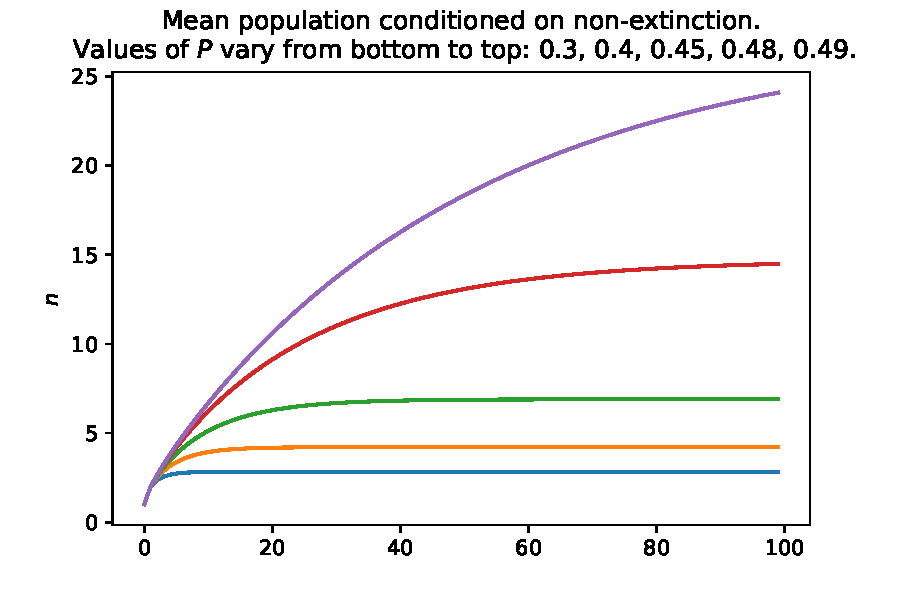
\includegraphics[width=0.78\textwidth]{figures/conditionalMean.pdf}
\caption{The conditional mean $(2p)^n/S_n$ against generation number $n$, with
$S_n$ obtained by iterating \cref{m:eq:SnIter}. From bottom to top,
$p=0.3,\,0.4,\,0.45,\,0.48,\,0.49$. Each curve approaches the constant $1/A(p)$;
the limiting values are $2.825$, $4.208$, $6.893$, $14.703$ and $27.476$,
obtained by iterating the recursion until $S_n/(2p)^n$ stabilises. The lowest
three have essentially converged by $n=100$, but the $p=0.49$ curve has reached
only $24.1$ of its limiting $27.5$ --- the near-critical slowdown analysed in
\ChA.}
\label{m:fig:condmean}
\end{figure}

Two further facts round out the quasi-stationary picture without proof. The
conditional variance also converges, to a constant depending on $p$ and $A(p)$
alone; the derivation is in \cref{m:app:variance}. And the convergence of the
first two moments is consistent with, but does not by itself prove, convergence
of the full conditional distribution; that is the content of the Yaglom theorem
quoted at the head of this subsubsection.
